\documentclass{beamer}
\usepackage[applemac]{inputenc}
\usepackage[spanish,activeacute]{babel}
\usepackage{amsmath}
\usepackage{amssymb}
\usepackage{latexsym}
\usepackage{listings}
\lstset{language=haskell, frame=single, tabsize=2}

\newcommand{\hpage}{$\lambda Page$}
\newcommand{\haskell}{\textsl{Haskell}}
\newcommand{\smalltalk}{\textsl{Smalltalk}}
\newcommand{\speech}[1]{}
\newcommand{\G}{\mathcal{G}}
\usetheme{DC}


\title{\hpage}
\author{\textsl{Fernando~Benavides}}
	
\institute{Departamento de Computaci�n, FCEyN,Universidad de Buenos Aires.}

\date{\today}

\begin{document}

\begin{frame}
	\titlepage
\end{frame}

\section{Introducci�n}
\subsection{Presentaci�n}
\begin{frame}
     \emph{El Orador}\\
     \begin{itemize}
       \item Fernando Benavides
	 \end{itemize}
	\pause
     \emph{El camino recorrido}\\
     \begin{itemize}
       \item Alumno de Computaci�n desde 2001
       \item Programador desde hace m�s de 10 a�os
       \item Programador \textsl{Funcional} desde hace 2 a�os
	\end{itemize}
	\pause
     \emph{La idea}\\
     \begin{itemize}
       \item Desarrollar una herramienta para los programadores funcionales como las que existen en el paradigma de orientaci�n a objetos
	\end{itemize}
\end{frame}

\subsection{Motivaci�n}
\begin{frame}[fragile]
	\frametitle{Trabajando en \haskell}
	\begin{columns}[c]
		\column{.5\textwidth}?`C�mo trabaja un desarrollador \haskell?
			\pause
			\begin{itemize}
				\item Crea o modifica m�dulos con su editor de texto favorito
				\pause
				\item Los compila utilizando \textsl{GHC}
				\pause
				\item Genera paquetes con \textsl{Cabal}
				\pause
				\item Para realizar pruebas, recurre a \textsl{GHCi}
			\end{itemize}
		\column{.5\textwidth}
			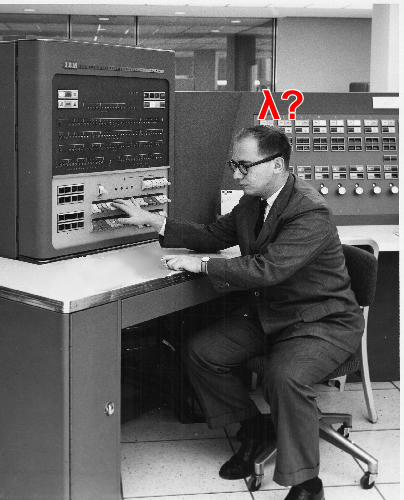
\includegraphics[height=.75\textheight]{pictures/photos/haskell}
		\end{columns}
\end{frame}
\begin{frame}[fragile]
	\frametitle{GHCi}
	\begin{columns}[c]
		\column{.5\textwidth}
			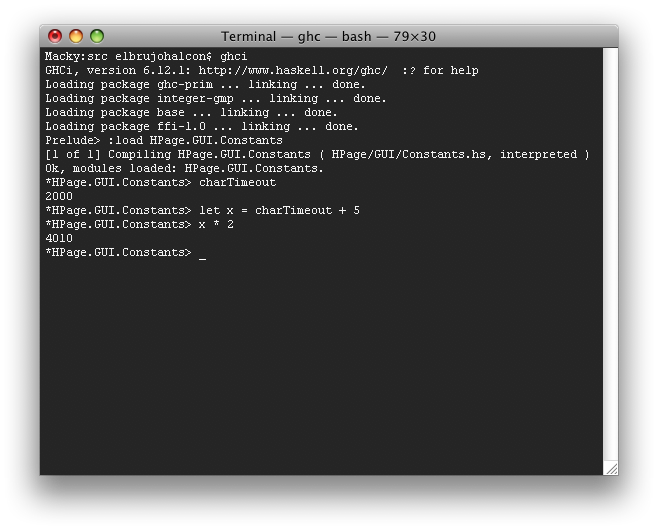
\includegraphics[width=\textwidth]{pictures/ghci}
		\column{.5\textwidth}
			\textsl{GHCi} permite:
			\begin{itemize}
				\item introducir c�digo para ejecutarlo y observar los resultados obtenidos
				\item definir expresiones y utilizarlas
				\item cargar m�dulos para utilizar sus funciones, tipos de datos, etc.
			\end{itemize}
	\end{columns}
\end{frame}
\begin{frame}[fragile]
	\frametitle{Trabajando con Lenguajes Orientados a Objetos}
	\begin{columns}[c]
		\column{.5\textwidth}
			
\includegraphics[width=\textwidth]{pictures/photos/java}
		\column{.5\textwidth}En cambio quienes programan en \textsl{Java}, \textsl{.NET} o \textsl{Smalltalk} cuentan con una \textsl{IDE} que provee
			\pause
			\begin{itemize}
				\item Autocompleci�n de c�digo
				\pause
				\item Compilaci�n autom�tica
				\pause
				\item Debugger integrado
				\pause
				\item Herramientas para \textsl{``micro-testing''}
			\end{itemize}
		\end{columns}
\end{frame}
\begin{frame}[fragile]
	\frametitle{``Micro-testing''}
	\begin{columns}[c]
		\column{.5\textwidth}
			El \textsl{Workspace} de \smalltalk\ permite:
			\begin{itemize}
				\item introducir c�digo para ejecutarlo, inspeccionarlo y  analizar los resultados obtenidos
				\item administrar varias paginas de texto
				\item crear objetos y utilizarlos
			\end{itemize}
		\column{.5\textwidth}
			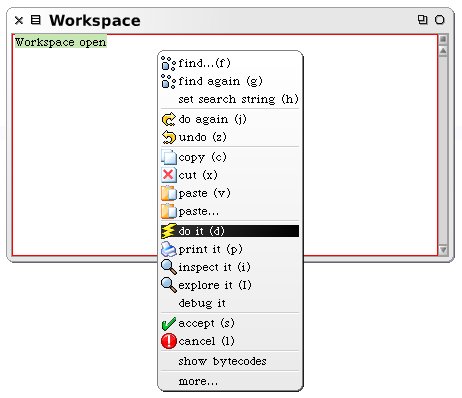
\includegraphics[width=\textwidth]{pictures/workspace}
	\end{columns}
\end{frame}


\section{Conociendo \hpage}
\begin{frame}
	\begin{center}
		{\Huge \emph{Conociendo \hpage}}
	\end{center}
\end{frame}
\subsection{Como el Workspace  de Smalltalk \ldots}
\begin{frame}[fragile]
	\frametitle{Como el Workspace  de Smalltalk \ldots}
	\hpage\ es similar al \textsl{Workspace} de \smalltalk\ pues permite al usuario
	\begin{itemize}
		\item Evaluar expresiones
		\item Detectar excepciones
		\item Administrar p�ginas de texto libre
		\item Intercalar expresiones y definiciones
	\end{itemize}
\end{frame}
\subsection{\ldots pero para Haskell}
\begin{frame}
	\frametitle{\ldots pero para Haskell}
	Pero, a su vez, por estar hecho para \haskell, presenta otros desaf�os
	\begin{itemize}
		\item \textsl{Lazy evaluation}
		\pause
		\item Expresiones puras vs. Expresiones con efectos
		\pause
		\item Administraci�n de m�dulos
	\end{itemize}
\end{frame}

\section{\hpage\ por Dentro}
\begin{frame}
	\begin{center}
		{\Huge \emph{\hpage\ por Dentro}}
	\end{center}
\end{frame}
\subsection{Desarrollo}
\begin{frame}
	\frametitle{Desarrollo de \hpage}
	\begin{itemize}
		\item \hpage\ est� desarrollado en \haskell
		\pause
		\item En gran parte est� desarrollado utilizando \hpage
		\pause
		\item Se conecta con \textsl{GHC} a trav�s de su API
		\pause
		\item Su interfaz gr�fica fue creada usando \textsl{wxHaskell}
		\pause
		\item Su alto grado de paralelismo se logra utilizando \textsl{eprocess}
	\end{itemize}
\end{frame}

\subsection{Arquitectura}
\begin{frame}
\frametitle{Arquitectura}
\begin{columns}[c]
	\column{.5\textwidth}Principales Requerimientos:
	\begin{itemize}
		\item Conexi�n con GHC
		\item Paralelismo
		\item Errores Controlados
		\item Presentaci�n de Resultados
	\end{itemize}
	\column{.5\textwidth}
		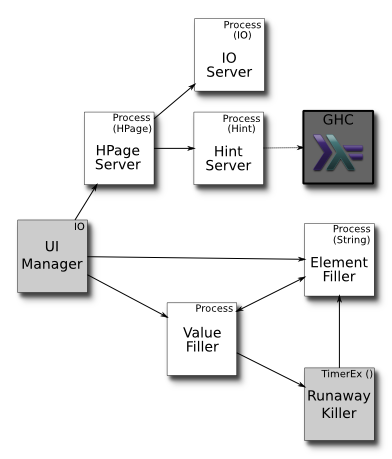
\includegraphics[height=.75\textheight]{pictures/architecture/00}
\end{columns}
\end{frame}
\begin{frame}[fragile]
\frametitle{Ejemplo de Interacci�n}
	Veremos c�mo interact�an estos componentes para evaluar la siguiente expresi�n:
	\begin{lstlisting}
		readFile "hpage.cabal" >>=
		    return . length . head . lines
	\end{lstlisting}
\end{frame}
\begin{frame}
\frametitle{Ejemplo de Interacci�n}
\begin{columns}[c]
	\column{.5\textwidth}\textsl{Procesos Involucrados:}
	\begin{itemize}
		\item \texttt{UI~Manager} \textbf{operando}
	\end{itemize}
	\column{.5\textwidth}
		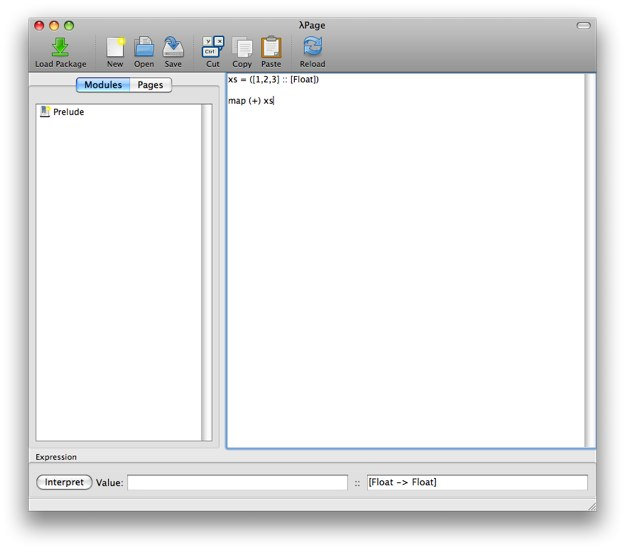
\includegraphics[height=.75\textheight]{pictures/architecture/01}
\end{columns}
\end{frame}
\begin{frame}
\frametitle{Ejemplo de Interacci�n}
\begin{columns}[c]
	\column{.5\textwidth}\textsl{Procesos Involucrados:}
	\begin{itemize}
		\item \texttt{UI~Manager} esperando
		\item \texttt{HPage~Server} \textbf{operando}
	\end{itemize}
	\column{.5\textwidth}
		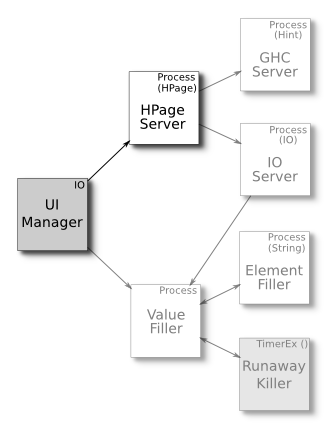
\includegraphics[height=.75\textheight]{pictures/architecture/02}
\end{columns}
\end{frame}
\begin{frame}
\frametitle{Ejemplo de Interacci�n}
\begin{columns}[c]
	\column{.5\textwidth}\textsl{Procesos Involucrados:}
	\begin{itemize}
		\item \texttt{UI~Manager} esperando
		\item \texttt{HPage~Server} esperando
		\item \texttt{GHC~Server} \textbf{operando}
	\end{itemize}
	\column{.5\textwidth}
		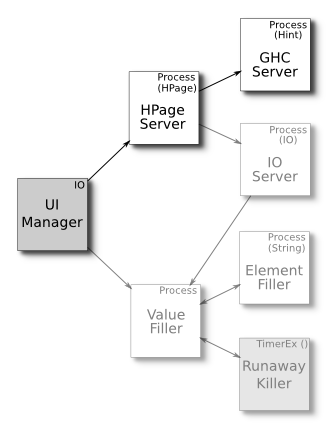
\includegraphics[height=.75\textheight]{pictures/architecture/03}
\end{columns}
\end{frame}
\begin{frame}
\frametitle{Ejemplo de Interacci�n}
\begin{columns}[c]
	\column{.5\textwidth}\textsl{Procesos Involucrados:}
	\begin{itemize}
		\item \texttt{UI~Manager} \textbf{operando}
		\item \texttt{IO~Server} \textbf{operando}
		\item \texttt{Value~Filler} esperando
	\end{itemize}
	\column{.5\textwidth}
		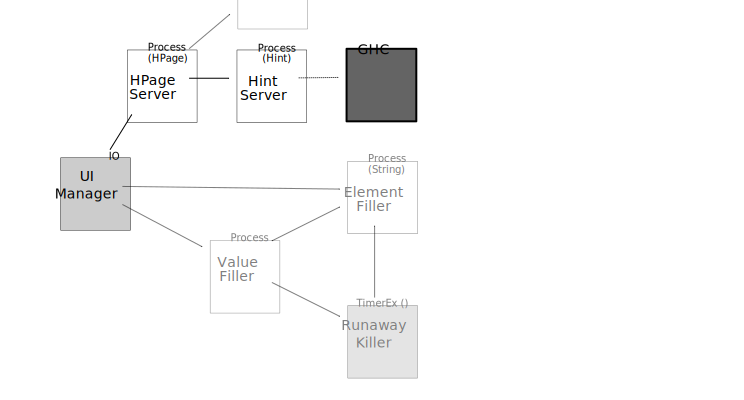
\includegraphics[height=.75\textheight]{pictures/architecture/04}
\end{columns}
\end{frame}
\begin{frame}
\frametitle{Ejemplo de Interacci�n}
\begin{columns}[c]
	\column{.5\textwidth}\textsl{Procesos Involucrados:}
	\begin{itemize}
		\item \texttt{UI~Manager} \textbf{operando}
		\item \texttt{Value~Filler} esperando
		\item \texttt{Element~Filler} \textbf{operando}
		\item \texttt{Runaway~Killer} \textbf{operando}
	\end{itemize}
	\column{.5\textwidth}
		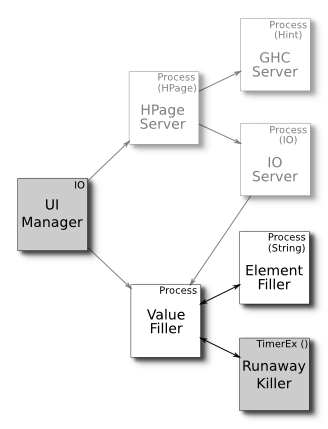
\includegraphics[height=.75\textheight]{pictures/architecture/05}
\end{columns}
\end{frame}
\begin{frame}
\frametitle{Ejemplo de Interacci�n}
\begin{columns}[c]
	\column{.5\textwidth}\textsl{Procesos Involucrados:}
	\begin{itemize}
		\item \texttt{UI~Manager} \textbf{operando}
	\end{itemize}
	\column{.5\textwidth}
		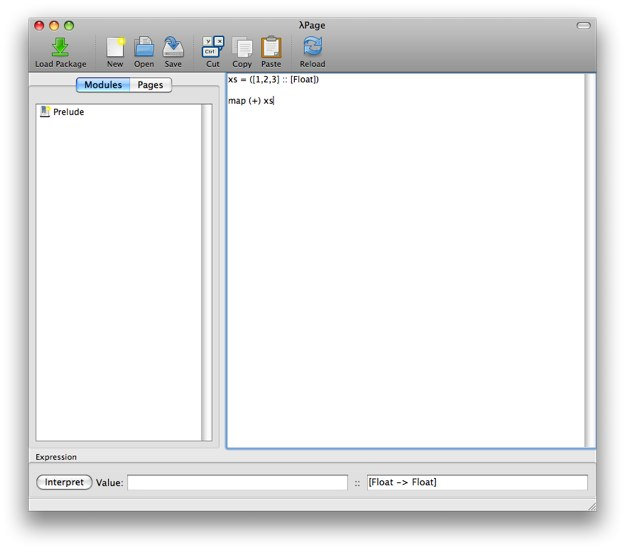
\includegraphics[height=.75\textheight]{pictures/architecture/01}
\end{columns}
\end{frame}



\section{Pr�ximos Pasos}
\begin{frame}
	\begin{center}
		{\Huge \emph{Pr�ximos Pasos}}
	\end{center}
\end{frame}
\subsection{Limitaciones}
\begin{frame}
	\frametitle{Limitaciones}
	\begin{itemize}
		\item M�s tipos \textsl{especiales}
			\begin{itemize}
				\item Tuplas
				\item Either
				\item Maybe
			\end{itemize}
		\pause
		\item Composici�n
			\begin{itemize}
				\item Listas de listas
				\item Acciones que generen listas
				\item Listas de acciones
			\end{itemize}
		\pause
		\item Nuevas visualizaciones
			\begin{itemize}
				\item M�s que un cuadro de texto
			\end{itemize}
	\end{itemize}
	\pause
	?`Qu� se puede hacer?
	\begin{itemize}
		\item Clase \texttt{Presentable}
	\end{itemize}
\end{frame}

\subsection{Trabajo a Futuro}
\begin{frame}
	\frametitle{Otras Herramientas}
	Con \hpage\ hemos acercado al desarrollador \haskell\ s�lo \textbf{una} de muchas herramientas:
			\begin{itemize}
				\item Mejores herramientas para TDD
				\item Refactoring
				\item An�lisis de Terminaci�n
				\item \ldots
			\end{itemize}
\end{frame}
\begin{frame}
	\frametitle{Otras Herramientas}
	\begin{columns}[c]
		\column{.5\textwidth}Con \hpage\ hemos acercado al desarrollador \haskell\ s�lo \textbf{una} de muchas herramientas:
			\begin{itemize}
				\item Mejores herramientas para TDD
				\item Refactoring
				\item An�lisis de Terminaci�n
				\item \ldots
			\end{itemize}
		\column{.5\textwidth}
			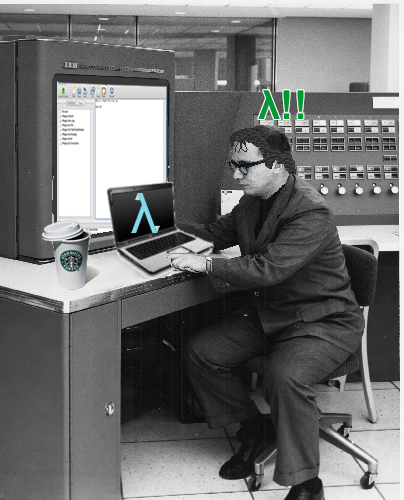
\includegraphics[height=.75\textheight]{pictures/photos/haskellcoolman}
		\end{columns}
\end{frame}

\begin{frame}
\frametitle{Agradecimientos / Preguntas}
	\begin{itemize}
		\item \textsl{Sitio Web de \hpage}:
		\begin{itemize}
			\item http://hpage.haskell.com
		\end{itemize}
		\item \textsl{\hpage\ en Github}
		\begin{itemize}
			\item http://github.com/elbrujohalcon/hPage
		\end{itemize}
		\item \textsl{Fernando Benavides en la Internet}
		\begin{itemize}
			\item http://profiles.google.com/greenmellon
		\end{itemize}
	\end{itemize}
\end{frame}
\end{document}